% ---------------------------------------------------------------------------
% §4.2 Experimental Results — Results bölümüne, kalibrasyon sonuçlarının
% (4.1) ardından eklenecek alt bölüm. Kalibrasyondaki gibi bold-başlıklı
% bulgu formatında. Figür yolları:
%   outputs/experiments/exp10_context_peacev3/paper_figs/
% Overleaf'e yüklerken figürleri kopyalayıp \includegraphics yollarını uyarla.
% ---------------------------------------------------------------------------

\subsection{Experimental Results}
\label{sec:exp-results}

This section reports the results of the political-structure experiment. All
estimates are within-persona paired contrasts between the threat (security)
and opportunity (peace) conditions over the full synthetic population.
Subgroup analyses use four respondent characteristics: age, education,
ethnic origin, and left--right self-placement. Respondents whose
characteristic is not reported are excluded from the corresponding
breakdown.

\textbf{Political structure moves both outcomes in the same direction.}
Moving the same protest event from an opportunity to a threat environment
lowers perceived movement legitimacy from 2.34 to 1.98 on the five-point
scale, a within-persona shift of $-0.35$ ($t = -12.1$, $p < .001$,
$d_z = -0.24$), and reduces the share of twins who would attend the march
from 22.8 to 6.7 percent, a shift of $-16.1$ percentage points
($t = -22.4$, $p < .001$, $d_z = -0.44$). The costly behavioral disposition
contracts proportionally far more than the evaluative judgment: the security
environment cuts expressed willingness to attend to less than a third of its
opportunity-condition level, while legitimacy declines but does not
collapse. Figure~\ref{fig:exp-main} summarizes the two contrasts.

\begin{figure}[t]
  \centering
  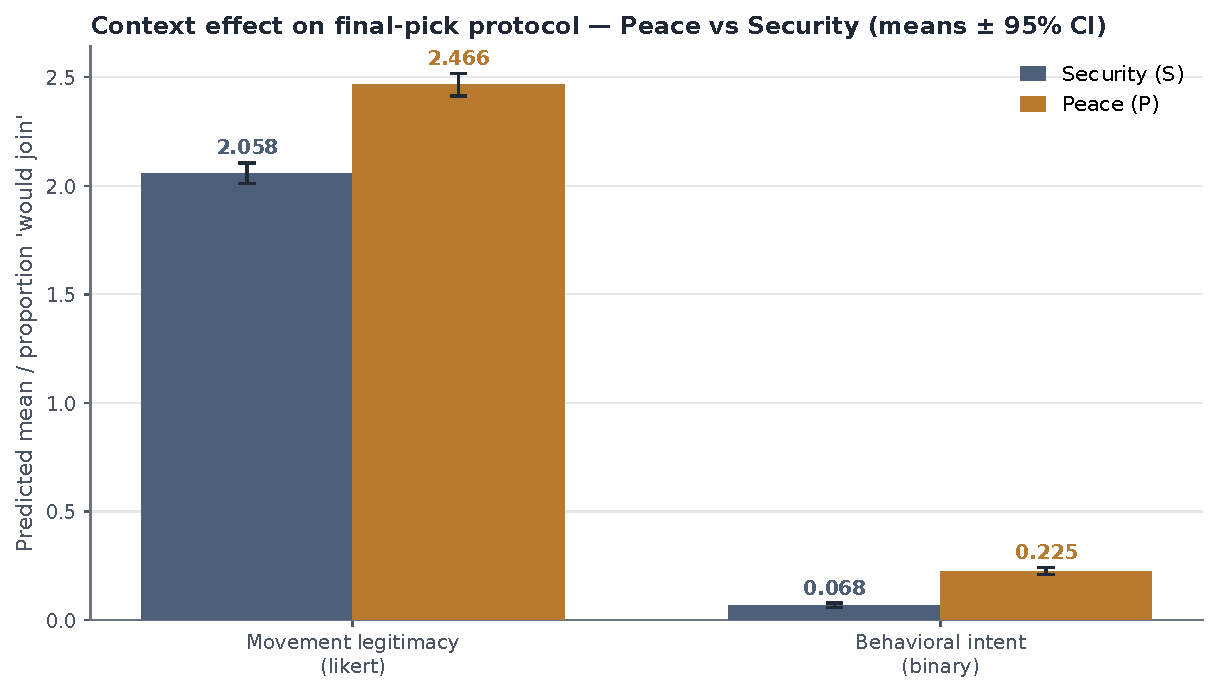
\includegraphics[width=.85\textwidth]{figures/fig_context_main.pdf}
  \caption{Political-structure effect on both outcomes. Points are condition
  means over the full synthetic population ($n = 2{,}615$) with 95\%
  confidence intervals; $p$-values are from within-persona paired
  $t$-tests.}
  \label{fig:exp-main}
\end{figure}

\textbf{Within each political structure, responses are stratified by
politics, ethnicity, and education.} In the opportunity condition, left-placed
twins rate legitimacy 0.47 points above the rest of the population and 55.8
percent of them would attend, against 13.9 percent among the remainder
($d = 0.98$). Kurdish twins rate legitimacy 0.19 points higher than
non-Kurdish twins ($p = .001$) and are substantially more willing to attend
(34.2 versus 19.6 percent, $d = 0.33$). Willingness to attend also rises
monotonically with education and is highest among twins aged 18--29. The
same ordering holds in the threat condition at uniformly lower levels: left
placement ($+0.60$ on legitimacy, $d = 0.53$) and Kurdish origin ($+0.25$,
$d = 0.22$) remain the strongest cleavages, and every one-way test across
the four breakdowns is significant except age on legitimacy.
Figures~\ref{fig:exp-peace-sub} and~\ref{fig:exp-security-sub} report the
subgroup means with the associated tests.

\begin{figure}[t]
  \centering
  \includegraphics[width=\textwidth]{figures/fig_peace_subgroup_signif.pdf}
  \caption{Opportunity (peace) condition: subgroup means and 95\% confidence
  intervals for both outcomes across the four breakdowns. Panel headers
  report the one-way test across subgroup levels (Welch $t$ for two-level
  breakdowns, $F$ otherwise); stars mark the one-vs-rest contrast for the
  focal categories (Kurdish; Left). Respondents with unreported
  characteristics are excluded.}
  \label{fig:exp-peace-sub}
\end{figure}

\begin{figure}[t]
  \centering
  \includegraphics[width=\textwidth]{figures/fig_security_subgroup_signif.pdf}
  \caption{Threat (security) condition: subgroup means, confidence
  intervals, and significance tests, as in
  Figure~\ref{fig:exp-peace-sub}.}
  \label{fig:exp-security-sub}
\end{figure}

\textbf{The size of the political-structure effect is itself politically
structured.} On legitimacy, the largest within-persona shift occurs at the
political center ($-0.44$), with smaller shifts on the left ($-0.26$) and
right ($-0.33$): the ideological poles hold relatively stable evaluations
across environments, while the center moves. On behavioral intent the
pattern reverses in a substantively informative way: the left shifts most
($-35.1$ points), the center shifts moderately ($-17.2$), and the right
barely moves ($-4.1$) because its willingness to attend is near the floor in
both conditions. Kurdish twins likewise shift more than non-Kurdish twins on
intent ($-22.9$ versus $-14.2$ points): the constituencies most willing to
mobilize under the opportunity structure are the ones with the most
mobilization to lose under threat. The full set of subgroup contrasts is
shown in Figure~\ref{fig:exp-forest}.

\begin{figure}[t]
  \centering
  \includegraphics[width=\textwidth]{figures/fig_context_effect_forest.pdf}
  \caption{Within-persona political-structure effect (threat minus
  opportunity) by subgroup, for both outcomes, in a single display. Squares
  are subgroup means of the paired difference with 95\% confidence
  intervals; the dashed line marks the population-level effect. Dark markers
  are significant at $p < .05$.}
  \label{fig:exp-forest}
\end{figure}

\textbf{Evaluations and dispositions respond to the environment, not only to
who is answering.} Because every twin answers under both political
structures, the estimates above cannot be produced by compositional
differences between conditions. The experiment therefore recovers, inside a
calibrated synthetic population, the conditional claim that motivated the
design: the same protest event, advanced by the same movement with the same
claim, elicits systematically weaker public legitimacy and sharply weaker
mobilization potential when it unfolds under threat rather than opportunity,
and the cost of the threat environment falls disproportionately on the
movement's most mobilizable publics.
